\documentclass[11pt,a4paper]{article}
\usepackage[T1]{fontenc}
\usepackage[utf8]{inputenc}
\usepackage[margin=24mm]{geometry}
\usepackage{lmodern,microtype,amsmath,amssymb,booktabs,tabularx,graphicx,placeins}
\usepackage[numbers,sort&compress]{natbib}
\usepackage{xcolor,algorithm,algpseudocode,capt-of,xurl}
\usepackage[hidelinks]{hyperref}
\providecommand*{\algorithmautorefname}{Algorithm}
\setlength{\emergencystretch}{2em}
\newcommand{\EAL}{\textsc{EAL}}
\newcommand{\given}{\mid}
\newcommand{\code}[1]{\texttt{#1}}
\title{Checked evidence and model-authored conclusions in API load testing:\\
  a complete six-model EAL/2 development pilot}
\author{}
\date{27 September 2026\\Development-results manuscript}
\begin{document}
\maketitle

\begin{abstract}
We analyse a completed development experiment in which six pinned language-model snapshots assessed the same 40 controlled API load-test cases under six prompt and tool conditions. All 1,440 assignments completed. A strict answer required selection of the correct report, matching scope, the three-way decision, complete failed and unknown check sets, and the recorded metrics. EAL/2 with MCP assessment produced 223 correct answers in 240 model--case assignments; explicit prose with an ordinary deterministic validator produced 219, while a JSON rendering of the EAL argument without assessment produced 166. These are repeated observations on 40 purposively reviewed cases, not 240 independent tasks. Four models scored 40/40 under both checked conditions. The remaining paired EAL-only/validator-only counts were 6/2 for GPT-4.1 nano and 3/3 for GPT-5.4 nano. All 17 EAL errors labelled unavailable evidence as a failed performance result. The ordinary validator produced 14 such errors and seven false claims of passing performance. In every model stratum, EAL/MCP had higher token-estimated cost and median trial time than the ordinary validator. The design bundles notation, MCP execution and checking, so it cannot identify a notation-specific benefit. The result supports a bounded account of checked evidence and model restatement in this finite development suite and specifies the controls needed for a held-out study.
\end{abstract}
\noindent\textbf{Keywords:} engineering argumentation; evidence acquisition; language models; paired development experiment; API load testing; assessment fidelity

\section{Question and evidential boundary}
An API performance judgement needs a report for the requested run, a usable observation, and a rule for interpreting its measurements. A fluent answer can preserve the measured p95 and still convert an unavailable report into a definitive pass or fail. Executable reasoning systems such as program-aided language models and solver-assisted formulations separate a model's proposal from a computational step \citep{gao2023,pan2023}. That separation does not ensure that a model communicates the computed result faithfully.

EAL/2 expresses a claim, scoped evidence, a versioned reasoning method and supporting arguments. The experiment supplied a fixed EAL argument rather than asking models to author one. Its \code{eal\_mcp} tool validated that argument, collected a selected report, evaluated the claim and returned an explanation. Five comparators separated a JSON rendering, three prose instructions, and explicit prose accompanied by an ordinary deterministic validator. The protocol fixes the tested source and environment, but the EAL arm still bundles notation, MCP transport and executable checking. The validator comparator therefore tests whether EAL's observed answer accuracy adds anything beyond an ordinary checker in this particular interaction, rather than isolating EAL syntax or a general argumentation semantics.

Our root claim is conditional: in this completed, purposively constructed development suite, both checked routes often preserved full decisions better than unchecked prompting, while the ordinary validator matched EAL on four model snapshots and EAL incurred a measured resource premium. This is an analysis of \href{https://github.com/emmett08/earl/actions/runs/36275725154}{GitHub Actions run 36275725154}, dispatched against commit \code{f8c629f49b5bef6c760de2029f6bc7db0e762a6f}. Its successful job retained \href{https://github.com/emmett08/earl/actions/runs/36275725154/artifacts/10916929645}{artifact 10916929645}, SHA-256 \code{0d1286e661eabb78470a2283d160979d4aae7221f98a086189ee7495124de018}. The repository labels the 40 reviewed cases as development-only and explicitly withholds confirmatory inference. We preserve that boundary throughout.

\section{Investigation and measurement}
\subsection{Evidence and assignment}
The protocol uses ten families, with four variants each: healthy, near-limit, slow, errors, incomplete, wrong-identity, stale, corrupt, conflicting and distractor. Each case contains a real local HTTP measurement run followed by recorded perturbations of the report catalogue. These cases exercise defined failure mechanisms; they are not a sample of naturally occurring production incidents. The independent reference derives its decision and check sets from the raw request rows without importing the collector or EAL evaluator. It classifies nine cases as supported, twelve as unsupported and nineteen as unavailable. An unavailable finding records inadequate identity, freshness, completeness, consistency or validity; it is not a measured failure of a performance threshold.

Every model received each arm for every case, producing $40\times6\times6=1{,}440$ assignments. The six exact snapshots were GPT-4.1, GPT-4.1 mini and nano dated 14 April 2025, and GPT-5.4, mini and nano dated 5 March or 17 March 2026 as recorded in the model matrix. The run used native tool transport and \emph{model} finalisation throughout. The model selected a report, invoked the available tool and authored the final status and measurements. A successful checker result did not automatically become the final answer. The retained ledger records 1,440 completed trials, no failed or unattempted assignments, and 2,889 model calls. The calls and underlying HTTP requests are cost and measurement events, not independent judgement tasks.

The EAL arm received a source argument and \code{assess\_load\_test}, which invoked MCP validation, collection, typed computation and explanation. \code{json\_prompt} received a JSON representation of the same argument as prompt text and direct report inspection. \code{plain\_brief}, \code{plain\_explicit} and \code{plain\_review} used distinct ordinary-language instructions and the same direct inspector. \code{plain\_validator} used the explicit prose task and direct inspection augmented with an ordinary deterministic checker that returned status, failed and unknown checks, and metrics. The JSON and prose arms did not execute EAL. All arms saw the same immutable case evidence, although their prompts and available operations differed.

\begin{figure}[htbp]
\centering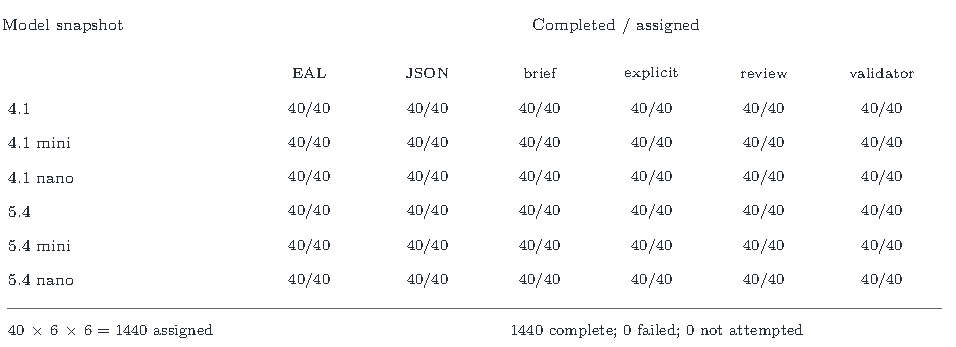
\includegraphics[width=\linewidth]{figures/fig1-assignment.pdf}
\caption{Complete assignment coverage across the six model snapshots and six arms. Each cell records 40 completed of 40 assigned cases. The same 40 cases recur in every cell; the 1,440 assignments do not represent 1,440 independent cases.}\label{fig:assignment}
\end{figure}

\subsection{Decision and scoring contract}
Let $V_c$ mean that the report for case $c$ meets the validity, identity, completeness, consistency and freshness checks. For an admissible report with $n_c$ attempted requests, the finite performance predicates are
\begin{equation}
  B_c=\left(n_c\geq100\right)\land
  \left(t_{c,(\lceil .95 n_c\rceil)}\leq200\,\mathrm{ms}\right)\land
  \left(e_c\leq .01\right),
  \label{eq:criterion}
\end{equation}
where $t_{c,(k)}$ is the $k$th ordered attempted-request latency and $e_c$ is the proportion of non-2xx or transport-failed attempts. The reference status is $\mathrm{unavailable}$ when $V_c$ fails, $\mathrm{supported}$ when $V_c\land B_c$, and $\mathrm{unsupported}$ when $V_c\land\neg B_c$. For $n_c>0$ and a finite latency limit $L$, the nearest-rank condition $t_{c,(\lceil .95n_c\rceil)}\leq L$ is equivalent to at least $\lceil .95n_c\rceil$ attempted latencies being at most $L$: the order statistic occupies that position if and only if the cumulative count reaches it. This arithmetic identity clarifies the two implementations' common numerical target. Test agreement between collector and independent reference remains executable evidence, not a machine-checked refinement proof or evidence that this criterion fits every engineering setting.

Write $Y_{mca}=1$ only when the completed final answer from model $m$, case $c$ and arm $a$ meets \emph{all} rubric components: selected report, bound service/build/run scope, status, complete failed and unknown check sets, and numeric measurements. A failed or unattempted assignment would contribute zero to the assigned denominator. We also examine status correctness and false support separately. A false-support event is a model answer of \code{supported} when the reference is either \code{unsupported} or \code{unavailable}; an unavailable-to-unsupported answer is a distinct false assertion of a measured failure. Explanation presence does not establish explanation quality.

For a model and paired arms $a,b$, the finite-suite difference is
\begin{equation}
 D_m(a,b)=\frac{1}{40}\sum_{c=1}^{40}(Y_{mca}-Y_{mcb})
          =\frac{n_{10}-n_{01}}{40},
 \label{eq:paired}
\end{equation}
where $n_{10}$ counts $a$-only correct cases and $n_{01}$ counts $b$-only correct cases. This paired table is the relevant descriptive unit; McNemar's matched-proportion framework motivates retaining discordant counts \citep{mcnemar1947}. We calculate no population $p$-value or confidence interval from these selected development cases. Reusing one case across six models does not create six sampled cases, and one stochastic session per case--model--arm combination does not estimate response variability.

\autoref{alg:audit-paired-run}, the archive-bound paired assessment audit, states the essential checks implemented by \code{analysis/analyse\_run.py}. It compares independently accumulated cells and pairs with the retained summary and emits a compact, de-identified assignment ledger. Its source and output are reviewable; no claim of formal verification of the Python implementation follows from the pseudocode.
\begin{algorithm}[t]
\caption{Audit the fixed archive and compute finite-suite paired outcomes}\label{alg:audit-paired-run}
\begin{algorithmic}[1]
\Require Archive $Z$; pinned digest $h$
\Ensure Audited cells and paired tables, or an integrity error
\If{$\Call{SHA256}{Z}\ne h$}
  \State \Return $\mathrm{integrity\_error}$
\EndIf
\State $(M,S,R)\gets\Call{ReadManifestSummaryTrials}{Z}$
\If{$\Call{Ids}{R}\ne\Call{Ids}{M}$ or $|R|\ne1440$}
  \State \Return $\mathrm{integrity\_error}$
\EndIf
\ForAll{$(m,a,c)$ in the declared model--arm--case product}
  \State $Y_{mca}\gets\Call{CompleteAndRubricCorrect}{R[m,a,c]}$
\EndFor
\ForAll{$(m,a,b)$ in declared paired comparisons}
  \State $(n_{11},n_{10},n_{01},n_{00})\gets\Call{PairCounts}{Y_{ma\cdot},Y_{mb\cdot}}$
  \If{$n_{11}+n_{10}+n_{01}+n_{00}\ne40$}
    \State \Return $\mathrm{integrity\_error}$
  \EndIf
\EndFor
\If{$\neg\Call{AgreesWithRetainedSummary}{S,Y,n_{11},n_{10},n_{01},n_{00}}$}
  \State \Return $\mathrm{integrity\_error}$
\EndIf
\State \Return audited aggregate and compact assignments
\end{algorithmic}
\end{algorithm}

\section{Observed outcomes}
\subsection{Complete answers}
Table~\ref{tab:correct} reports the strict outcome using the assigned denominator of 40 within each snapshot and arm. All cells completed, so no attrition adjustment changes the numerator. The EAL route produced 223 fully correct answers across the six model strata; the ordinary validator produced 219. The four full and mini models obtained 40/40 under both checked routes. GPT-4.1 nano obtained 27/40 with EAL and 23/40 with the validator, while GPT-5.4 nano obtained 36/40 with both. Unchecked prompt-only totals were 166 for JSON, 170 for brief prose, 171 for explicit prose and 169 for review prose across the same repeated model--case records. The total of 240 per arm describes coverage, not an independent-case sample size.

\begin{table}[t]
\centering\small
\caption{Fully correct model-authored answers out of 40 assigned cases per model and arm. ``Validator'' is the ordinary deterministic checker paired with explicit prose.}\label{tab:correct}
\begin{tabular}{lrrrrrr}
\toprule
Model snapshot & EAL/MCP & JSON & Brief & Explicit & Review & Validator\\
\midrule
GPT-4.1 & 40 & 29 & 35 & 34 & 35 & 40\\
GPT-4.1 mini & 40 & 25 & 26 & 25 & 26 & 40\\
GPT-4.1 nano & 27 & 5 & 7 & 9 & 4 & 23\\
GPT-5.4 & 40 & 38 & 39 & 37 & 39 & 40\\
GPT-5.4 mini & 40 & 38 & 38 & 38 & 40 & 40\\
GPT-5.4 nano & 36 & 31 & 25 & 28 & 25 & 36\\
\midrule
Repeated model--case records & 223 & 166 & 170 & 171 & 169 & 219\\
\bottomrule
\end{tabular}
\end{table}

\begin{figure}[htbp]
\centering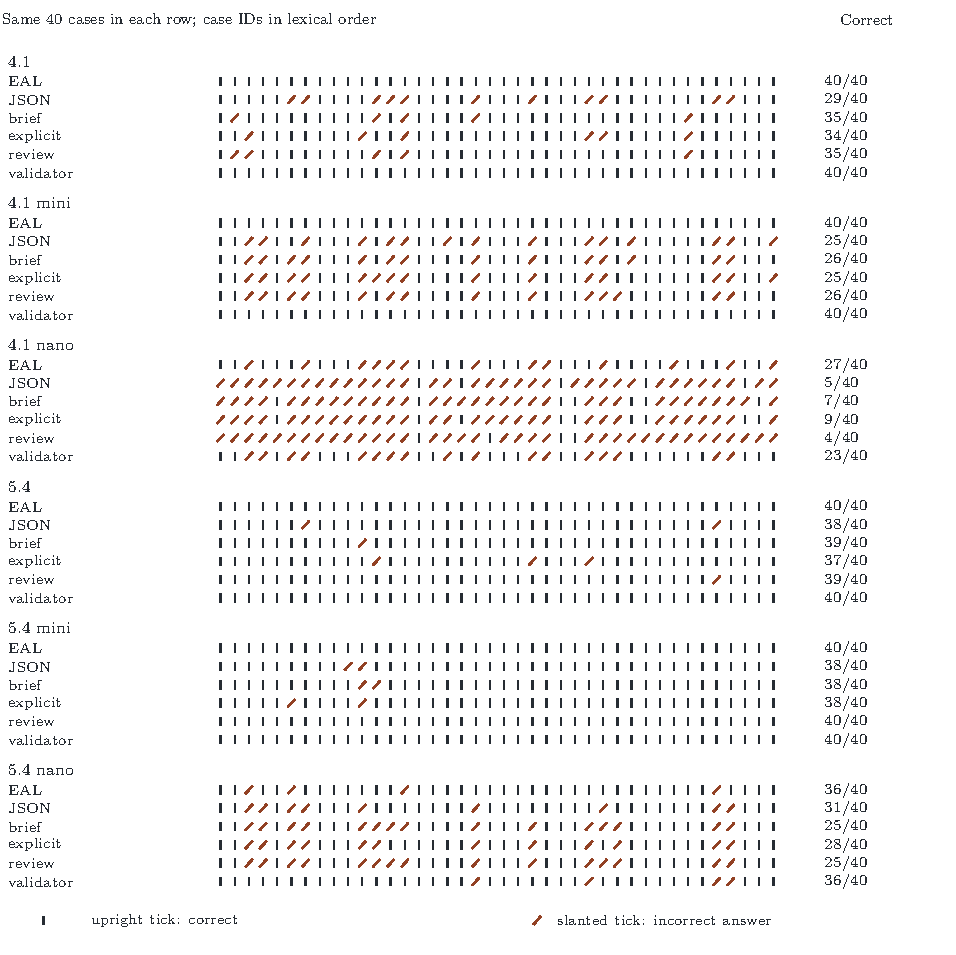
\includegraphics[width=\linewidth]{figures/fig2-correctness.pdf}
\caption{Strict full-answer results for each of the 36 model--arm cells, with a fixed denominator of 40 in every cell. Directly labelled marks preserve the individual model strata; proximity of two marks does not imply equivalent performance in a new case population.}\label{fig:correctness}
\end{figure}

The paired tables in Table~\ref{tab:paired} show why differences between cell totals require case alignment. For GPT-4.1 nano, EAL alone was correct on six cases and the validator alone on two, a net $4/40$ on this suite. GPT-5.4 nano had three discordances in each direction, despite equal totals. The EAL--JSON comparison gave larger EAL-only counts for the GPT-4.1 family, whereas GPT-5.4 nano included one JSON-only case. The four models at 40/40 under both checked routes provide no observed difference on these cases; they do not establish equivalence elsewhere.

\begin{table}[t]
\centering\small
\caption{Paired strict correctness. Each four-number entry is both correct / EAL only / comparator only / both incorrect, always over the same 40 cases.}\label{tab:paired}
\begin{tabular}{lcc}
\toprule
Model snapshot & EAL versus validator & EAL versus JSON\\
\midrule
GPT-4.1 & 40/0/0/0 & 29/11/0/0\\
GPT-4.1 mini & 40/0/0/0 & 25/15/0/0\\
GPT-4.1 nano & 21/6/2/11 & 5/22/0/13\\
GPT-5.4 & 40/0/0/0 & 38/2/0/0\\
GPT-5.4 mini & 40/0/0/0 & 38/2/0/0\\
GPT-5.4 nano & 33/3/3/1 & 30/6/1/3\\
\bottomrule
\end{tabular}
\end{table}

\begin{figure}[htbp]
\centering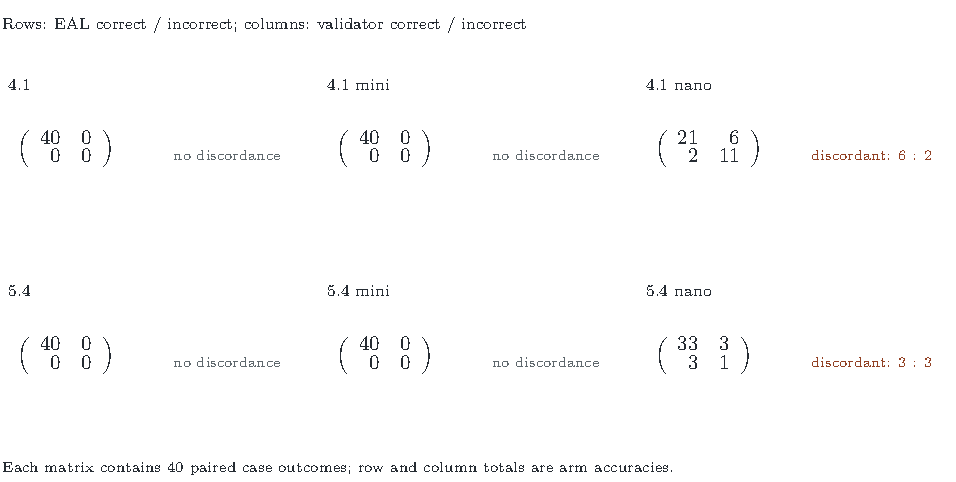
\includegraphics[width=\linewidth]{figures/fig3-paired.pdf}
\caption{Six paired EAL--validator correctness matrices, each resolving the same 40 cases into both-correct, EAL-only, validator-only and both-incorrect outcomes. The finite-suite net difference is the signed discordance count divided by 40. The separate EAL--JSON counts appear in Table~\ref{tab:paired}.}\label{fig:paired}
\end{figure}

\subsection{The status error after checking}
The reference assigns nineteen of the 40 cases to unavailable evidence. Every one of the 17 EAL full-answer errors was an unavailable-to-unsupported status change: thirteen with GPT-4.1 nano and four with GPT-5.4 nano. The selected report, scope, failed and unknown check sets, and metrics in these errors agreed with the reference; the final model-authored status did not. The ordinary validator's 21 full-answer errors consisted of fourteen unavailable-to-unsupported changes and seven unavailable-to-supported changes, all of the latter in GPT-4.1 nano. Thus zero EAL false-support events is narrower than perfect epistemic caution: an unavailable-to-unsupported statement still claims a measured failure that the evidence cannot establish.

The checker agreed with the independent reference in these cases. The model's final restatement changed its meaning. In the five families whose variants include unavailable evidence, EAL's full-correct counts across the 24 repeated model--case records per family were 22 conflicting, 21 corrupt, 21 incomplete, 18 stale and 21 wrong-identity; the ordinary validator scored 18, 22, 20, 19 and 20 respectively. Both checked routes scored 24/24 in each of healthy, distractor, errors, near-limit and slow. Each family contains only four distinct cases, so the family pattern diagnoses this suite rather than estimating a general failure rate.

\begin{figure}[htbp]
\centering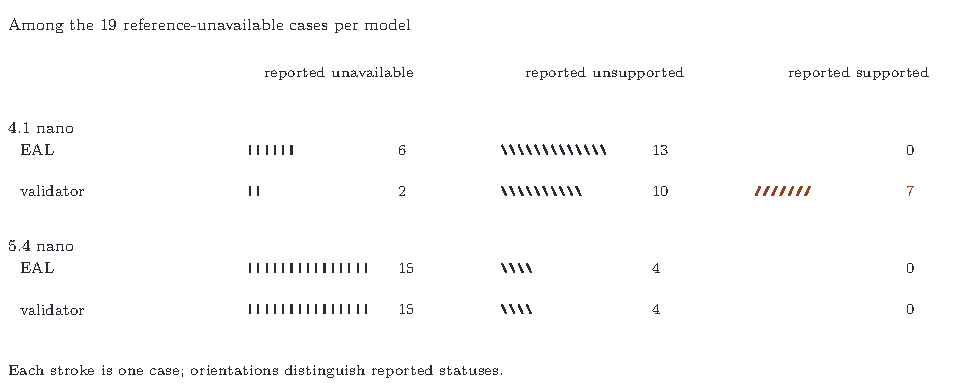
\includegraphics[width=\linewidth]{figures/fig4-false-support.pdf}
\caption{Final status assigned to the nineteen reference-unavailable cases in each nano snapshot's two checked arms. An unavailable-to-unsupported answer asserts failure without admissible evidence; an unavailable-to-supported answer asserts a pass. Each stroke denotes one model--case--arm response.}\label{fig:status-errors}
\end{figure}
\FloatBarrier

\subsection{Time and measured cost}
The run estimated model-call cost from recorded usage and its frozen rate schedule; it is not an invoice and excludes any unpriced external infrastructure. All 2,889 calls have known estimated cost in the retained summary. Across the six model strata, EAL/MCP cost \$1.46336 and the ordinary validator \$1.19735. EAL's known-cost ratio to the validator is between 1.17 and 1.26 within each stratum. Median attempted-trial time was 8.47--10.70 seconds with EAL and 3.92--6.11 seconds with the validator; the six within-model median ratios lie between 1.70 and 2.28. The complete run's estimated model cost across all six arms was \$8.3231. These values measure this runner, tool route and provider sessions. They do not imply a stable price or throughput ordering under other providers, concurrency settings or workload mixes.

\begin{figure}[htbp]
\centering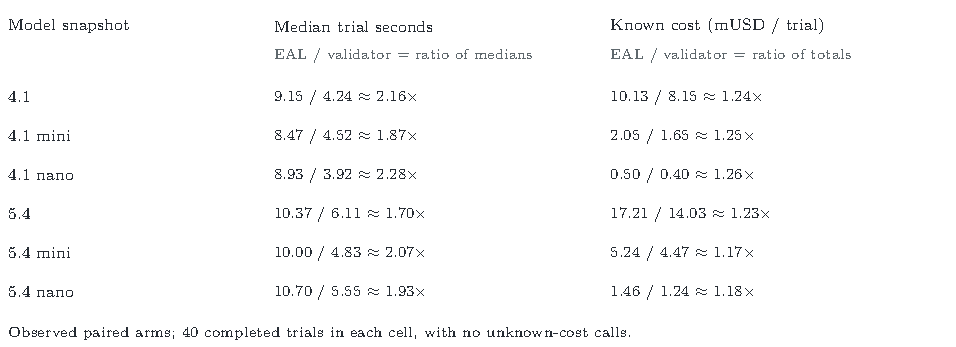
\includegraphics[width=\linewidth]{figures/fig5-resource.pdf}
\caption{Median attempted-trial time and known token-estimated model cost per trial for EAL and the ordinary validator in each snapshot, with within-model ratios. The cost is a 40-trial cell total divided by 40; the time is a median, so the two scales are not additive or exchangeable. Strict correctness appears in Table~\ref{tab:correct}.}\label{fig:resources}
\end{figure}

\FloatBarrier
\section{Interpretation and rival explanations}
The strongest observed distinction is access to an executable checker. The EAL and ordinary-validator routes both exposed a deterministic decision and outscored unchecked prompts on several snapshots. Their equality on four models and close, mixed discordances on the two nano snapshots challenge a claim that EAL's notation uniquely caused better model answers. The experiment does not factor notation and checking independently: the EAL route changes prompt representation, tool protocol and reasoned packet; the validator supplies a conventional checked packet after direct collection. Model tier, exact prompt, tool-output presentation, status vocabulary and interaction length can each contribute to the observed pattern.

The completed assignment ledger avoids the attrition problem in earlier pilots, but it does not remove selection or response variation. Cases were deliberately reviewed and reused; their class balance is engineered, with nineteen unavailable cases. Each model--case--arm combination has one realised stochastic conversation. The arm order and provider conditions may influence responses. Distinct model snapshots and prices are separate strata, not six exchangeable draws from a model population. Repeated case exposure across contrasts also makes a pooled significance calculation inappropriate. The reference adjudicator is implemented independently of collector and EAL evaluation, yet both follow the authored engineering criteria, so agreement does not establish that those criteria capture all operational risk.

The observed checker-to-answer gap suggests a concrete design test: retain a checked host status as the authoritative output used for an action, and let the model supply an optional explanation without rewriting that status. This run used model finalisation; it did not evaluate that alternative. A follow-up should predeclare a practical difference, generate new held-out cases, hold transport and evidence presentation constant while crossing notation and checking as separate factors, randomise condition order, and repeat independent model sessions within case. Case-level paired outcomes and model-level heterogeneity would then determine a suitable uncertainty analysis. An authoring task would be needed to test whether engineers or models can formulate the EAL argument correctly; this fixed-source experiment cannot answer it.

\section{Reproduction and conclusion}
The archive includes the assignment manifest, completed trials, original case measurements, model calls and summary. The companion \code{analysis/analyse\_run.py} verifies the archive digest, source revision, manifest coverage, every model--arm--case identity, summary cell totals, known call costs and paired tables before writing \code{results/aggregate.json} and \code{results/assignments.csv}. The compact ledger omits model transcripts and original HTTP rows; the exact run artifact is needed for a full independent audit. Its GitHub retention expires on 26 October 2026 unless copied to a durable research archive. The new article and its five figure sources reside in a separate directory and leave \code{paper/manuscript.tex} intact.

Within the 40 reviewed cases, deterministic checking supplied useful decision information, yet a model sometimes changed \code{unavailable} to a definitive conclusion when it wrote the final answer. EAL/MCP and the ordinary validator performed similarly on most model strata, with EAL taking more measured time and estimated model cost. The next investigation can isolate notation, checking and finalisation on held-out cases; this complete pilot provides the observed failures and comparison conditions from which to design it.

\bibliographystyle{plainnat}
\bibliography{references}
\end{document}
